\documentclass{llncs}
\usepackage{color}
\usepackage{soul}
\usepackage{cite}
\usepackage{array}
\usepackage{listings}
\usepackage{graphicx}
\usepackage{amsfonts}

\usepackage{url}
\newcommand{\starpar}[1]{\par{\footnotesize $\star$ \hl{#1}\par}}

\lstset{basicstyle=\scriptsize,breaklines=true,breakindent=60pt,xleftmargin=20pt,numberstyle=\tiny,numbersep=5pt,language=C}

\begin{document}

\title{Recovering OpenSSL ECDSA Nonces Using the \textsc{Flush+Reload} Cache Side-channel Attack}

\maketitle

\begin{abstract}
\end{abstract}

\section{Introduction}
Elliptic curves cryptography~\cite{miller85use,koblitz87elliptic} is a collection of public key cryptographic methods that rely on the computational
intractability of the elliptic curves discreet logarithm problem.
In a nutshell, given an elliptic curve over a finite field and two points on the curve~$G$ and~$H$,
the discreet logarithm problem is finding a scalar $k$ such that $H=kG$.

Elliptic curve cryptography offers a higher encryption strength per key-bit than similar methods based on 
discreet logarithms over finite field or on number factoring.
Consequently, elliptic curves cryptography uses significantly shorter keys and offers faster operations
than other methods, contributing to the rising popularity of elliptic curves cryptography.

The Elliptic Curve Digital Signature Algorithm (ECDSA)~\cite{johnson01elliptic,fips186,ansi962} is a standard
digital signature algorithm based on elliptic curves.
The core operation of the ECDSA algorithm is multiplying a point on the elliptic curve by a randomly
or pseudo-randomly chosen secret nonce.
The confidentiality of the nonce is paramount for the security of the algorithm.
Past research indicates that partial exposure of nonce bits can be exploited for efficient attacks on the secret key~\cite{nguyen03insecurity,brumley11remote}.

OpenSSL~\cite{openssl} is a cryptographic software package that implements ECDSA.
When using elliptic curves over a binary field $\mathbb{F}_{2^m}$, OpenSSL uses the 
Montgomery ladder~\cite{montgomery87speeding,joye03montgomery} algorithm for multiplying the point by the nonce.
One of the advantages of the Montgomery ladder is that it has a very regular behaviour performing
the same sequence of operations for each nonce bit, irrespective of the value of the bit.
This regular behaviour makes it more resilient to side-channel attacks~\cite{joye03montgomery,okeya00elliptic}.

While the operations performed by the algorithm are regular, their targets depend on the value of the bits of the nonce.
To apply the operations to the respective targets, the OpenSSL implementation uses a conditional branch based on the value of the bit.
By tracing this branch an attacker can recover the values of the nonce bits and, consequently, break the cryptosystem.

In this paper we present our 
use the \textsc{Flush+Reload} cache side-channel attack~\cite{yarom13flush}
to trace the branch in the OpenSSL implementation.
\textsc{Flush+Reload} relies on a security weakness in the IA-32 and X86-64 architectures that allows processes
to monitor other processes read and execute access to shared memory pages.
Our attack program monitors access to both arms of the conditional branch and uses the information
collected from these probes to reconstruct the nonce.

The paper also presents new information on the limitation of the \textsc{Flush+Reload} attack.
We discuss spatial limitations, affecting the distance between multiple probes, and 
temporal limitations, affecting the probe resolution.

\starpar{Analysis of partial nonce exposure?}

The rest of this paper is organised as follows.
The next section presents background information on elliptic curves, ECDSA, the Montgomery ladder and the \textsc{Flush+Reload} attack.
Section~\ref{sec:attack} describes our attack on the OpenSSL implementation of ECDSA.
The results of the attack are analysed in Section~\ref{sec:results}.
We discuss the implications of the attack and suggest techniques for mitigation in Section~\ref{sec:discussion}.
Section~\ref{sec:related} presents related research.
\section{Preliminaries}\label{sec:background}
\subsection{ECDSA}
\subsection{The Montgomery Ladder}
\subsection{The \textsc{Flush+Reload} attack}
\section{Attacking OpenSSL ECDSA}\label{sec:attack}
OpenSSL is one of the most common open-source cryptographic libraries.
It provides a set of cryptographic services, including public and shared key encryption 
algorithms and public key signature algorithms.

OpenSSL's implementation of ECDSA uses the Montgomery ladder algorithm for scalar multiplication
on the Elliptic Curve.
We use this implementation to demonstrate that na{\"\i}ve implementations of the Montgomery ladder are
susceptible to the \textsc{Flush+Reload} attack.

Listing~\ref{lst:openssl} shows the relevant section of the implementation of the Montgomery ladder in OpenSSL version 1.0.1e.
The bits of the multiplication scalar are stored in the word array \texttt{scalar->d}.
The outer loop, at lines~268 to~286 traverses over the words representing the scalar.
The inner loop, at lines~271 to~284 traverses the bits in each word.
Line~273 tests the bit. 
For each bit the implementation executes a group add followed by a group double.
If the bit is set, the implementation uses lines~275 and~276.
For clear bits it uses lines~280 and~281.

\begin{lstlisting}[numbers=left,firstnumber=268,float=htb,caption=OpenSSL Implementation of the Montgomery Ladder,label=lst:openssl]
for (; i >= 0; i--)
{
    word = scalar->d[i];
    while (mask)
    {
        if (word & mask)
        {
            if (!gf2m_Madd(group, &point->X, x1, z1, x2, z2, ctx)) goto err;
            if (!gf2m_Mdouble(group, x2, z2, ctx)) goto err;
        }
        else
        {
            if (!gf2m_Madd(group, &point->X, x2, z2, x1, z1, ctx)) goto err;
            if (!gf2m_Mdouble(group, x1, z1, ctx)) goto err;
        }
        mask >>= 1;
    }
    mask = BN_TBIT;
}
\end{lstlisting}

As the listing demonstrates, the Implementation is very regular.
For each bit, the implementation executes exactly the same sequence of operations.
The only differences between set and clear bit are the lines that invoke these operations.
Our attack exploits this difference.
The attack probes the cache lines used by OpenSSL to identify the branch taken by the \texttt{if}
statement in line~273.
From this information we can deduce the value of the bit and by repeating the attack throughout
the execution of the scalar multiplication we can recover most of the bits of the nonce.


The mapping of source lines to cache lines in our build of OpenSSL is depicted in Diagram~\ref{dgm:memory}.
The machine code created from source lines~273 to~282 covers the virtual memory address range 0x0812130C
to 0x081213e8.
This range spans four cache lines, marked $A$, $B$, $C$ and $D$.
The attacks observes the sequence of cache access made by the processor when executing the code.


\begin{figure}[htb]
\centering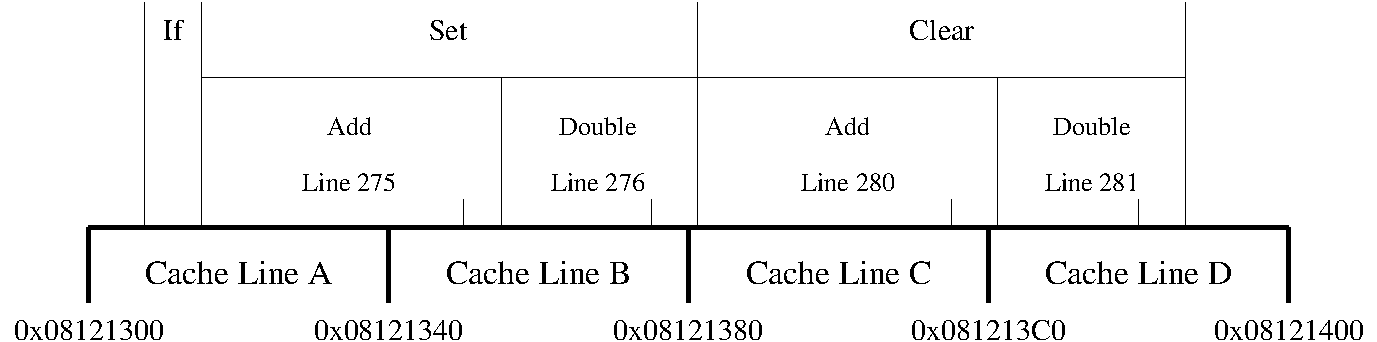
\includegraphics[width=\columnwidth]{images/memory}
\caption{Mapping from Source Code to Memory\label{dgm:memory}}
\end{figure}


\starpar{required, actual and observed cache access sequences}

The \texttt{if} statement at line~273 is executed for each bit.  
The code of this statement is in cache line $A$, hence this line is accessed when processing of a bit starts.
For set bit, the processing continues with source line~275, which maps to cache lines~$A$ and~$B$.
The actual call to the group add function occurs at address 0x08121347.
(See mark in Diagram~\ref{dgm:memory}.)
After a delay for computing the group add, execution continues in cache line~$B$ to process the return value and 
to invoke the group doubling function.
The group doubling function returns to cache line~$B$ and execution leaves the \texttt{if} body at cache line~$D$.

Hence, the sequence of cache line accesses required for a set bit is: $A$, $B$, \textit{add}, $B$, \textit{double}, $B$, $D$.
Similarly, for a clear bit, the sequence is: $A$, $C$, \textit{add}, $C$, $D$, \textit{double}, $D$.

Processor optimisations may add otherwise unrequired cache line accesses.
The spatial prefetching optimisation~\cite{intel12optimization} pairs adjacent cache lines and tries to bring both cache lines
when there is a miss on one of the pair's line.
For example, when there is a cache miss on cache line~$A$, the spatial prefetcher may attempt to prefetch cache line~$B$
and vice versa.

Another optimisation that can cause additional cache line access is speculative execution~\cite{uht95disjoint}.
With speculative execution, the processor follows both \hl{arms} of a conditional branch before evaluating
the condition.
When the condition is evaluated, the processor commits to the pre-processed computation of the correct \hl{arm},
disposing of the computation done for the other \hl{arm}. 
In the case of OpenSSL this means that even before evaluating the bit, 
the processor may start processing both line~275 and line~280, triggering memory loads from cache lines~$A$, $B$ and $C$.




\section{Results}\label{sec:results}

\starpar{Test architecture}
\starpar{Curve - sect571k1}
\starpar{Operation times}
\starpar{Choice of slot size}
\starpar{Example of results}
\starpar{Number of lost bits}
\section{Discussion}\label{sec:discussion}
\starpar{LLL attack}
\starpar{Expected number of observed signatures to break key}
\starpar{Smaller keys are more resilient}~\cite{walter04longer}
\starpar{Mitigation, Dan Bernstein NaCL}
\section{Related Work}\label{sec:related}
\section{Conclusions}

%\starpar{Bitcoin uses ECDSA}~\cite{nakamoto--bitcoin}

\bibliographystyle{splncs}
\bibliography{Euro2014}

\end{document}

